\documentclass[aspectratio=169,handout]{beamer}
% \usepackage[utf8]{inputenc}
\usetheme{metropolis}
\usecolortheme{orchid}
\usepackage{amsmath}
\usepackage{amssymb}
\usepackage{amsthm}
\usepackage{multirow}
\usepackage[ruled]{algorithm2e}
\usepackage{mathtools}
\usepackage{caption}
\usepackage{epstopdf}
\usepackage{hyperref}
\setbeamerfont{footnote}{size=\tiny}

\usepackage{tikz}
\usetikzlibrary{mindmap,shadows,tikzmark,positioning,arrows.meta}

% Information boxes
\newcommand*{\info}[4][16.3]{%
  \node [ annotation, #3, scale=0.65, text width = #1em,
          inner sep = 2mm ] at (#2) {%
  \list{$\bullet$}{\topsep=0pt\itemsep=0pt\parsep=0pt
    \parskip=0pt\labelwidth=8pt\leftmargin=8pt
    \itemindent=0pt\labelsep=2pt}%
    #4
  \endlist
  };
}

\tikzset{%
  >={Latex[width=2mm,length=2mm]},
  % Specifications for style of nodes:
            base/.style = {rectangle, rounded corners, draw=black,
                           minimum width=4cm, minimum height=1cm,
                           text centered, font=\sffamily},
  activityStarts/.style = {base, fill=blue!30},
       startstop/.style = {base, fill=red!30},
    activityRuns/.style = {base, fill=green!30},
         process/.style = {base, minimum width=2.5cm, fill=orange!15,
                           font=\ttfamily},
}
\renewcommand\textbullet{\ensuremath{\bullet}}
\newcommand\scalemath[2]{\scalebox{#1}{\mbox{\ensuremath{\displaystyle #2}}}}
\newcommand{\norm}[1]{\left\lVert#1\right\rVert}

%%% Bibliography
\usepackage[citestyle=numeric,style=numeric,backend=biber,doi=false,isbn=false,url=false]{biblatex}
\addbibresource{references.bib}

%%% Suppress biblatex annoying warning
\usepackage{silence}
\WarningFilter{biblatex}{Patching footnotes failed}

%%% new theorems %%%%%%%%%%%%%%%%%%%%%%%%%%%%%%%%%%%%%%%%%%%%%%%%%%%%%%%%%%%%%%
\theoremstyle{definition}
\newtheorem{mydef}{Definition}

\theoremstyle{plain}
\newtheorem{mylemma}{Lemma}[section]
\newtheorem{mytheorem}{Theorem}[section]
\newtheorem{myproposition}{Proposition}[section]
\newtheorem{myproblem}{Problem}[section]
\newtheorem{mydefinition}{Definition}[section]
\newtheorem{myassumption}{Assumption}[section]

\theoremstyle{remark}
\newtheorem{myremark}{Remark}[section]

\newcounter{saveenumi}
\newcommand{\seti}{\setcounter{saveenumi}{\value{enumi}}}
\newcommand{\conti}{\setcounter{enumi}{\value{saveenumi}}}

\resetcounteronoverlays{saveenumi}

\title{Controles}
\subtitle{Clase 1: Introducción}
\author{Gerardo Becerra, Ph.D.}
\institute{Pontificia Universidad Javeriana\\ Departamento de Electrónica}
\date{Enero 22, 2020}

\begin{document}

\frame{\titlepage}	

% \frame{\tableofcontents}

\section{Presentación del Curso}
\begin{frame}[<+->]\frametitle{Descripción General del Curso}
\begin{itemize}
  \item El curso está dedicado al diseño e implementación de sistemas de control de entrada sencilla - salida sencilla en los dominios continuo y discreto.
  \item Se estudian procedimientos de análisis y diseño de controladores en el dominio del tiempo y la frecuencia.
  \item Se plantean los problemas fundamentales en el diseño de controladores: estabilidad, robustez y optimización.
  \item Se desarrollan proyectos en los que se implementan sistemas de control mediante:
  \begin{itemize}
    \item Construcción de modelos
    \item Diseño de la estrategia de control
    \item Implementación de la solución
    \item Validación de la solución.
  \end{itemize}
  \item Es prerequisito para el énfasis en Control y Automatización de pregrado y para asignaturas coterminales de maestría en el área de control automático.
\end{itemize}
\end{frame}

\begin{frame}[c]\frametitle{Objetivos del Curso}
\begin{itemize}
  \item Posicionar el control de sistemas en el contexto de automática.
  \item Definir y analizar especificaciones de desempeño de un sistema de control lineal e invariante.
  \item Modificar la respuesta dinámica de sistemas mediante sistemas de control.
  \item Seleccionar un controlador y sus parámetros óptimos para un problema dado.
  \item Reconocer y plantear alternativas de solución a los problemas básicos de control.
\end{itemize}
\end{frame}

\begin{frame}[<+->]\frametitle{Estrategias Pedagógicas del Curso}
\begin{itemize}
  \item Asignación de lecturas para estudio individual anterior y posterior a la clase.
  \item Exposiciones teóricas por parte del profesor (sesiones teóricas).
  \item Desarrollo de proyectos de aplicación (sesiones prácticas).
  \item Uso de herramientas de simulación y diseño de controladores.
\end{itemize}
\end{frame}

\begin{frame}[c]\frametitle{Actividades de Evaluación del Curso}
\centering
\begin{tabular}{c|c|c}
  \textbf{Componente}     & \textbf{Fecha}    & \textbf{Valor}\\
  \hline
  Examen parcial & Semana 9 & 30\% \\
  Examen final & Semana 17 & 30\% \\
  Talleres & Semana 16 & 20\% \\
  Tareas & Permanente & 20\%
\end{tabular}
\end{frame}

\begin{frame}[<+->]\frametitle{Contenidos Generales del Curso}
\textbf{Capítulo 1: Introducción al Control:}
\begin{itemize}
  \item Semana 1: 
  \begin{itemize}
    \item Introducción a la automatización: estructura jerárquica, dominios de control.
    \item Definiciones y términos asociados a los sistemas de control.
    \item Estructura de un sistema de control de lazo cerrado.
    \item Definición de bloques y variables
  \end{itemize}
  \item Semana 2:
  \begin{itemize}
    \item Especificaciones de desempeño.
    \item Modelo en espacio de estados y función de transferencia.
    \item Respuesta en el tiempo (FOL, FOLPDT, SO, resumen).
    \item Error en estado estacionario.
    \item Estabilidad.
  \end{itemize}
  \seti
\end{itemize}
\end{frame}

\begin{frame}[<+->]\frametitle{Contenidos Generales del Curso (cont)}
\textbf{Capítulo 2: Sintonización de Controladores:}
\begin{itemize}
  \conti
  \item Semana 3:
  \begin{enumerate}
    \item Acciones de control y controladores.
    \begin{itemize}
      \item Controladores de dos posiciones (ON-OFF).
      \item Controladores de tres términos: P, PI, PID.
    \end{itemize}
  \end{enumerate}
  \item Semana 4:
  \begin{enumerate}
    \item Criterios clásicos de sintonización (no óptimos):
    \begin{itemize}
      \item Modelos aproximados FOPDT.
      \item Métodos de Ziegler-Nichols, Cohen-Coon.
    \end{itemize}
    \item Criterios de sintonización óptima:
    \begin{itemize}
      \item Índices de desempeño.
      \item Sintonía por criterios IAE, ITAE, ISE.
    \end{itemize}
  \end{enumerate}
  \item Semana 5: Sesión de Matlab:
  \begin{itemize}
    \item Síntesis de controladores: método matemático por igualación de funciones características.
  \end{itemize}
  \seti
\end{itemize}
\end{frame}

\begin{frame}[<+->]\frametitle{Contenidos Generales del Curso (cont)}
\textbf{Capítulo 3: Diseño de compensadores por lugar geométrico de las raíces (LGR) y respuesta en frecuencia:}
\begin{itemize}
  \conti
  \item Semana 6:
  \begin{enumerate}
    \item Diseño de compensadores por LGR.
    \item Aproximación de polos dominantes.
  \end{enumerate}
  \item Semana 7:
  \begin{enumerate}
    \item Diseño de compensador en adelanto.
    \item Diseño de compensador en atraso.
    \item Diseño de compensador en adelanto-atraso.
  \end{enumerate}
  \seti
\end{itemize}
\end{frame}

\begin{frame}[<+->]\frametitle{Contenidos Generales del Curso (cont)}
\begin{itemize}
  \conti
  \item Semana 8: Diseño en el dominio de la frecuencia:
  \begin{itemize}
    \item Respuesta en frecuencia: diagramas de Bode, márgenes de fase y ganancia.
    \item Compensador en adelanto.
  \end{itemize}
  \item Semana 9: \textbf{Examen parcial.}
  \item Semana 10: Sesión de Matlab
  \begin{enumerate}
   \item Diseño de compensador en atraso.
   \item Diseño de compensador en adelanto-atraso.
  \end{enumerate}
  \item Semana 11: Sesión de Matlab
  \seti
\end{itemize}
\end{frame}

\begin{frame}[<+->]\frametitle{Contenidos Generales del Curso (cont)}
\textbf{Capítulo 4: Sistemas de control en tiempo discreto:}
\begin{itemize}
  \conti
  \item Semana 12: Sesión de Matlab
  \item Semana 13: Elementos de un sistema de control digital
  \begin{enumerate}
    \item Diagrama de bloques.
    \item Sistemas de datos muestreados.
    \item Funciones de transferencia.
    \item Correspondencia entre los planos $s$ y $z$.
    \item Presentación de proyecto.
  \end{enumerate}
  \seti
\end{itemize}
\end{frame}

\begin{frame}[<+->]\frametitle{Contenidos Generales del Curso (cont)}
\begin{itemize}
  \conti
  \item Semana 14: Controladores discretos
  \begin{itemize}
    \item Médotos de discretización de controladores.
    \begin{itemize}
      \item PID discreto.
      \item Transformación backward, forward, bilineal.
    \end{itemize}
    \item Diseño de controladores digitales
    \begin{itemize}
      \item Diseño por LGR en el plano $z$
    \end{itemize}
  \end{itemize}
  \item Semana 15, 16: Sesión de Matlab - Implementación de Algoritmos.
  \item Semana 17: Entrega de proyecto.
  \item Semana 18: \textbf{Examen final.}
  \seti
\end{itemize}
\end{frame}

\begin{frame}[c]\frametitle{Bibliografía del Curso}
\small
\textbf{Texto guía:}
\begin{itemize}
  \item Dorf, R. C., Bishop, (2011). Sistemas de control moderno. Pearson Prentice Hall.
\end{itemize}
\textbf{Otras referencias:}
\begin{itemize}
  \item Franklin, G. F., Powell, J. D., \& Workman, M. L. (2006). Digital control of dynamic systems. Menlo Park: Addison-wesley.
  \item Golnaraghi, F., \& Kuo, B. C. (2010). Automatic control systems. Wiley.
  \item CHEN Chi-Tsong. ANALOG AND DIGITAL CONTROL SYSTEM DESIGN: Transfer-Function,State-Space, and Algebraic Methods. Philadelphia: Saunders College, 1993.
  \item SMITH Carlos A. and CORRIPIO Armando. PRINCIPLES AND PRACTICE OF AUTOMATIC PROCESS CONTROL - 2nd. Edition. New York: John Wiley and Sons. 1997.
\end{itemize}
\end{frame}

\begin{frame}[<+->][c]\frametitle{Declaración de los Reglamentos}
\footnotesize
\begin{itemize}
  \item 113. Constituyen faltas graves:
  \begin{itemize}
    \footnotesize
    \item d. El fraude en actividades, trabajos y evaluaciones académicos y la posesión o utilización de material no autorizado en los mismos.”
  \end{itemize}
  \item “118. Adicional a la sanción disciplinaria, el fraude en actividades, trabajos y evaluaciones académicos se sancionará académicamente con la pérdida de la asignatura, la cual será calificada con nota definitiva de cero punto cero (0.0)”
  \item “120. Además de la sanción disciplinaria, el plagio o la suplantación en una evaluación académica, en exámenes preparatorios, en trabajo de grado y tesis, se sancionarán académicamente con la pérdida de la asignatura la cual será calificada con nota definitiva de cero punto cero (0.0).”
  \item “67. Evaluación supletoria es aquella que remplaza otra evaluación académica que el estudiante no pudo presentar oportunamente, por razones debidamente justificadas por escrito ante el Director del Programa. Dicha justificación deberá presentarse en un plazo no superior a los cinco días hábiles siguientes a la fecha de la evaluación no presentada.”
\end{itemize}
\end{frame}

\begin{frame}[c]\frametitle{Comunicación durante el curso}
\begin{itemize}
  \item Discord: \url{https://discordapp.com/download}
  \item Enlace de invitación al servidor privado: \url{https://discord.gg/R5XnvFM}
  \item Contenidos del curso.
  \item Trabajos propuestos.
  \item Discusiones y preguntas.
\end{itemize}
\end{frame}

\section{Fundamentos de Sistemas de Control}

\begin{frame}[<+->][c]\frametitle{Control de Sistemas - Contexto General}
  \textbf{Automática:}
  \begin{itemize}
    \item Ciencia que estudia los métodos y procedimientos que permiten la sustitución del operador humano por uno artificial, en una tarea previamente programada.
  \end{itemize}
  \textbf{Automatización:}
  \begin{itemize}
    \item Es la realización de tareas y funciones mediante máquinas de funcionamiento autónomo, sin la intervención directa del hombre.
  \end{itemize}
\end{frame}

\begin{frame}[c]\frametitle{Control de Sistemas - Importancia}
\textbf{Por qué es importante el control?}
\begin{itemize}
  \item En robótica: \href{https://www.youtube.com/watch?v=wlkCQXHEgjA}{(video)} \href{https://www.youtube.com/watch?v=_sBBaNYex3E}{(video)}
  \item En la industria automotriz: \href{https://www.youtube.com/watch?v=rbki4HR41-4}{(video)}
  \item En vehículos autónomos: \href{https://www.youtube.com/watch?v=tlThdr3O5Qo}{(video)}
  \item En la industria aeronáutica: \href{https://www.youtube.com/watch?v=GrP3jHuLQ9o}{(video)}
\end{itemize}
\end{frame}

\begin{frame}[<+->][c]\frametitle{Control de Sistemas - Introducción}
\begin{itemize}
  \item Ingenieros $\rightarrow$ crean productos para ayudar a las personas.
  \item Entender, modelar y controlar materiales y fuerzas de la naturaleza.
  \item Ingeniería de sistemas de control:
  \begin{itemize}
    \item Área de la ingeniería que busca entender, modelar y controlar segmentos del ambiente, llamados \textbf{sistemas}.
    \item Basada en los principios de teoría de retroalimentación, análisis de sistemas lineales.
    \item Fuertes fundamentos matemáticos y gran aplicabilidad en diversas áreas.
  \end{itemize}
\end{itemize}
\end{frame}

\begin{frame}[<+->][c]\frametitle{¿Qué es un sistema?}
\begin{center}
  \includegraphics[width=12cm]{images/planeSystem.png}
\end{center}  
\end{frame}

\begin{frame}[<+->][c]\frametitle{¿Qué es un sistema?}
\begin{center}
  \includegraphics[width=12cm]{images/biologySistem.png}
\end{center}  
\end{frame}

\begin{frame}[<+->][c]\frametitle{¿Qué es un sistema?}
\begin{center}
  \includegraphics[width=12cm]{images/socialNetwork.png}
\end{center}  
\end{frame}

\begin{frame}[<+->][c]\frametitle{Sistema}
\begin{itemize}
  \item Interconexión de componentes, dispositivos o subsistemas.
  \item Proceso que toma unas entradas y las transforma en salidas.
  \begin{center}
    \includegraphics[width=6cm]{images/sistema.png}
  \end{center}
  \item Relación entrada - salida: representa la relación causa - efecto del proceso.
  \item Existe una frontera que separa los componentes internos del mundo externo.
  \item Enfoque sistemático para analizar el comportamiento: modelos matemáticos.
\end{itemize} 
\end{frame}

\begin{frame}[<+->][c]\frametitle{Sistema de Control}
\begin{itemize}
  \item Interconexión de componentes que forman una configuración que provee una respuesta deseada.
  \item Sistema de control de lazo abierto: Usa un \textbf{controlador} y un \textbf{actuador} para obtener la respuesta del proceso deseada.
  \begin{center}
    \includegraphics[width=8cm]{images/openloopcontrol.png}
  \end{center}  
  \item Sistema de control de lazo cerrado: Utiliza una medida adicional de la salida para compararla con la respuesta deseada.
  \begin{center}
    \includegraphics[width=10cm]{images/closedloopcontrol.png}
  \end{center}  
\end{itemize}
\end{frame}

\begin{frame}[<+->][c]\frametitle{Sistema de Control}
  \vspace*{-0.2cm}
  \begin{center}
    \includegraphics[width=10cm]{images/closedloopcontrol2.png}
  \end{center}
  \vspace*{-0.7cm}
  \begin{itemize}
    \item Referencia (set-point): valor deseado de la variable controlada.
    \item Variable controlada: cantidad o condición que se mide y controla. Normalmente es la salida del sistema.
    \item Variable manipulada: cantidad o condición que el controlador modifica para afectar el valor de la variable controlada.
    \item Perturbación: señal externa que ocasiona que la variable de control se desvíe del punto de control.
  \end{itemize}
\end{frame}

\begin{frame}[<+->][c]\frametitle{Sistema de Control}
  \vspace*{-0.2cm}
  \begin{center}
    \includegraphics[width=10cm]{images/closedloopcontrol2.png}
  \end{center}
  \vspace*{-0.7cm}
  \begin{itemize}
    \item Ruido de medida: señal externa que contamina la medición hecha con el sensor sobre la variable controlada.
    \item Error: Diferencia entre la referencia y la medición obtenida mediante el sensor.
  \end{itemize}
\end{frame}

\begin{frame}[c]\frametitle{Sistemas de Control - Ejemplos: Vehículos autónomos}
  \begin{center}
    \includegraphics[width=8cm]{images/controlsystem_example1.png}
  \end{center}
\end{frame}

\begin{frame}[c]\frametitle{Sistemas de Control - Ejemplos: Operador humano en el lazo de control}
  \begin{center}
    \includegraphics[width=9cm]{images/controlsystem_example2.png}
  \end{center}
\end{frame}

\begin{frame}[c]\frametitle{Sistemas de Control - Ejemplos: Ingresos en una nación}
  \begin{center}
    \includegraphics[width=10cm]{images/controlsystem_example3.png}
  \end{center}
\end{frame}

\begin{frame}[c]\frametitle{Diseño de Sistemas de Control}
  \begin{columns}
    \begin{column}{0.4\textwidth}
       \textbf{Objetivo:} Obtener la configuración, especificaciones e identificación de los parámetros clave del sistema propuesto para satisfacer los requerimientos.
    \end{column}
    \begin{column}{0.6\textwidth}
      \begin{center}
        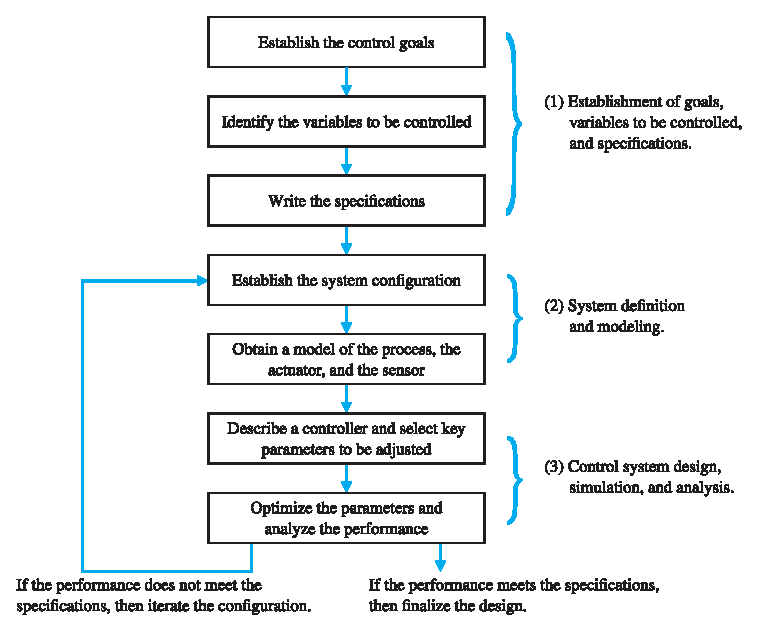
\includegraphics[width=8cm]{images/controlsystemdesign.eps}
      \end{center}
    \end{column}
  \end{columns}
\end{frame}

\begin{frame}[c]\frametitle{Taller - Sistemas de Control}
\begin{enumerate}
  \item Describa sensores típicos que puedan usarse para medir las siguientes variables:
  \begin{itemize}
    \item Posición lineal
    \item Posición rotacional
    \item Temperatura
    \item Presión
    \item Fuerza
    \item Flujo de líquido
    \item Campo magnético terrestre
  \end{itemize}
  \item Describa actuadores típicos que puedan convertir las siguientes variables:
  \begin{itemize}
    \item Energía eléctrica en energía mecánica
    \item Deformación mecánica en energía eléctrica
    \item Energía química en energía cinética
    \item Calor en energía eléctrica
  \end{itemize}
  \seti
\end{enumerate}
\end{frame}

\begin{frame}[c]\frametitle{Taller - Sistemas de Control (cont)}
\begin{enumerate}
  \conti
  \item Una cámara con foco automático ajusta la distancia entre el lente y el sensor usando un rayo infrarojo para determinar la distancia al objetivo. Realice un bosquejo del diagrama de bloques de éste sistema de control especificando los diferentes componentes y señales. Explique brevemente su operación.
  \seti
\end{enumerate}
\end{frame}

\begin{frame}[c]\frametitle{Taller - Sistemas de Control (cont)}
\begin{columns}
  \begin{column}{0.5\textwidth}
    \begin{enumerate}
      \conti
      \item Considere el péndulo invertido mostrado en la figura. El objetivo es mantener el péndulo en la posición vertical ($\theta = 0$) en la presencia de disturbios. Realice el bosquejo del diagrama de bloques del sistema de control. Identifique el proceso, sensor, actuador y controlador.
    \end{enumerate}
  \end{column} 
  \begin{column}{0.5\textwidth}
   \centering
   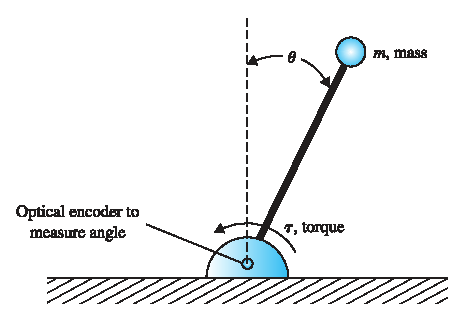
\includegraphics[width=6cm]{images/invertedpendulum.eps}
  \end{column} 
\end{columns}
\end{frame}

\end{document}